\documentclass[12pt]{article}
\usepackage{fullpage}
\usepackage{hyperref}
\usepackage{hanging}
\usepackage{perltex}
\usepackage{verbatim}
\usepackage[parfill]{parskip}    % Activate to begin paragraphs with an empty line rather than an indent
% The following is needed in order to make the code compatible
% with both latex/dvips and pdflatex.
\ifx\pdftexversion\undefined
\usepackage[dvips]{graphicx}
\else
\usepackage[pdftex]{graphicx}
\DeclareGraphicsRule{*}{mps}{*}{}
\fi


\title{Integration Test Plan for Mashbot} 

\author{George D'Andrea \and Andrew Gall \and Josiah Kiehl \and
  Cody Ray \and Vito Salerno}
\date{\today}


\newcommand{\CoreTestCases}[8]{
\begin{hangparas}{0.25in}{1}
Feature: #1 #2 \\
	#1 a #2  #7 multiple services \\
	As a client \\
	#8

\end{hangparas}

}

\begin{document}

\begin{titlepage}
\maketitle
\end{titlepage}

\section*{Revision History}
\begin{tabular}{|p{2in}|l|l|l|}
  \hline
  \textbf{Name} & \textbf{Date} & \textbf{Reason for Changes} & \textbf{Version} \\
  \hline \hline
  George D'Andrea, Andrew Gall, Josiah Kiehl, Cody Ray, Vito
  Salerno & 9 February 2010 & Initial Version & 1.0 \\
  \hline
\end{tabular}

\clearpage
\tableofcontents
\clearpage

\section{Introduction}
\subsection{Background}
This document provides the high level testing requirements for the Mashbot Campaign Manager and Publishing and Aggregation Platforms.  These tests will be implemented as behavioral tests that will be automatically run every time a feature is added to prevent regression.
\subsection{References}
\begin{itemize}
\item \href{http://mashbot.heroku.com/doc/Design.pdf}{Design.pdf}
\item \href{http://mashbot.heroku.com/doc/Testplan.pdf}{Testplan.pdf}
\item \href{http://mashbot.heroku.com/doc/Requirements.pdf}{Requirements.pdf}
\end{itemize}
\subsection{Definitions and Acronyms}

\section{Approach and Constraints}
\subsection{Objectives}
To assure integrity of the overall structure of the Mashbot Campaign Manager and Publishing and Aggregation Platform.
\subsection{Structure}

The Integration Test Plan shall contain test cases that verify
interoperability of design architecture components specified in
section 2.2 ”Architecture” of the Mashbot Design Document. The
following figure depicts this high-level system architecture.

\begin{centering}
\includegraphics{uml/teststructure.1}
\end{centering}

The test cases shall provide automatically testable scenarios that
focus on a single type of interaction between two design components.

Each scenario shall consist of a precondition, an action and a
postcondition for the scenario. The precondition shall describe the
state of the software before the tested action occurs. This may
require the test case implementation to artificially construct data
structures on both sides of the interface. The action defines how the
integration test will be triggered by running a method from one of the
two components. The postcondition is the desired state of the software
after the tested action. This is what should be tested in the test
case implementation to determine success or failure.  To automate
integration testing, each test case must:

\begin{itemize}
\item be self contained with appropriate setup and tear-down
  mechanisms
\item be runnable from a script or test suite
\item not require any user interaction while running
\item provide a single pass or fail result.
\end{itemize}


\subsection{Constraints}
\begin{itemize}
\item External APIs are not to be relied upon for testing, so these content sources will have to be mocked out for integration testing purposes.
\end{itemize}
\section{Assumptions and Exclusions}
\subsection{Assumptions}
\begin{itemize}
\item External APIs are assumed to have 100\% uptime
\item Each individual tests assume the rest of the service is working properly
\end{itemize}
\subsection{Exclusions}
\begin{itemize}
\item There will be no testing of External API calls, as they are assumed to be working.
\end{itemize}
\section{Entry and Exit Criteria}
\subsection{Entry Criteria}
\begin{itemize}
\item All lower level tests pass, including behavioral tests, and unit tests.
\item The hardware meets the specifications outlined in the Requirements Document.
\end{itemize}
\subsection{Exit Criteria}
\begin{itemize}
  \item All top priority tests pass | success
  \item At least one top priority test fails | failure
\end{itemize}

\section{Testing Participants}
\subsection{Roles and Responsibilities}
\begin{itemize}
\item Campaign Manager Test Lead: Josiah Kiehl
\item Publishing and Aggregation Platform Test Lead: Andrew Gall
\item Testers: Josiah Kiehl, Andrew Gall, Cody Ray, Vito Salerno, Nick D'Andrea
\end{itemize}

\subsection{Training Requirements}
Testers should have general familiarity with the Campaign Manager and Publishing and Aggregation Platform. They should also be familiar with either Chrome, Firefox, Safari, or Internet Explorer web browsers.

\subsection{Problem Reporting}
Issues will be reported via the issue tracker on http://github.com/codyaray/mashbot/issues and will be assigned to the proper development team from there.
\subsection{Progress Reporting}
Regressions and failures will be reported to the respective team lead when they are discovered. Successes are assumed and will not be further reported.

\section{Test Cases}

\subsection{Publishing and Aggregation Platform}

\subsubsection{Feature: Push Status}
	\CoreTestCases{Push}{Status}{Twitter}{Facebook}{And I have filled in at 
	least the status field in the object model}{And I have not filled in at 
	  least the status field in the object model}{to}{I want to be able to get 
		the ids for each individual status posted to each service that I 
		  specify.}

\subsubsection{Feature: Pull Status}
	\CoreTestCases{Pull}{Status}{Twitter}{Facebook}{}{}{from}{I want to be able 
	  to get a status from each service that I specify.}

\subsubsection{Feature: Edit Status}
	\CoreTestCases{Edit}{Status}{Twitter}{Facebook}{And I have filled in at 
	 least the relevant ids for each service  And I have filled in the status 
	   field in the object model}{And I have not filled in at least the status 
		 field in the object model or all relevant ids for each specified 
		   service are not present}{to}{I want to be able to get the ids for 
			 each edited status post for each service that I specify.}

\subsubsection{Feature: Delete Status}
	\CoreTestCases{Delete}{Status}{Twitter}{Facebook}{And I have filled in the 
	  status  ids for services which you would like to delete statuses 
		from.}{And I have not filled in status ids for all services which I 
		  would like to delete statuses from.}{from}{I want to be able to get 
			the ids for each deleted status post for each service that I 
			  specify.}

\subsubsection{Feature: Push Blog}
	\CoreTestCases{Push}{Blog}{Blogger}{Tumblr}{And I have filled in at least 
	the text and title fields in the object model}{And I have not filled in at 
	  least the text and title fields in the object model}{to}{I want to be able 
		to get the ids for each individual blog posted to each service that I 
		  specify.}

\subsubsection{Feature: Pull Blog}
	\CoreTestCases{Pull}{Blog}{Blogger}{Tumblr}{}{}{from}{I want to be able to 
	  get a blog entry from each service that I specify.}

\subsubsection{Feature: Edit Blog}
	\CoreTestCases{Edit}{Blog}{Blogger}{Tumblr}{And I have filled in at least 
	 the relevant ids for each service  And I have filled in the text and 
	   title fields in the object model}{And I have not filled in at least the 
		 text and title fields in the object model or all relevant ids for each 
		   specified service are not present}{to}{I want to be able to get the 
			 ids for each edited blog post for each service that I specify.}

\subsubsection{Feature: Delete Blog}
	\CoreTestCases{Delete}{Blog}{Blogger}{Tumblr}{And I have filled in the 
	  blog  ids for services which you would like to delete bloges 
		from.}{And I have not filled in blog ids for all services which I 
		  would like to delete bloges from.}{from}{I want to be able to get 
			the ids for each deleted blog post for each service that I 
			  specify.}

\subsubsection{Feature: Push Picture}
	\CoreTestCases{Push}{Picture}{Picasa}{Facebook}{And I have filled in at 
	least the picture, title, and album fields in the object model}{And I have 
	  not filled in at least the picture, title, and album fields in the object model}{to}{I want to 
		be able to get the ids for each individual status posted to each service 
		  that I specify.}

\subsubsection{Feature: Pull Picture}
	\CoreTestCases{Pull}{Picture}{Picasa}{Facebook}{}{}{from}{I want to be able 
	  to get a status from each service that I specify.}

\subsubsection{Feature: Edit Picture}

	\CoreTestCases{Edit}{Picture}{Picasa}{Facebook}{And I have filled in at 
	 least the relevant ids for each service  And I have filled in the 
	   picture, title, and album fields in the object model}{And I have not filled in at least the 
		 picture, title, and album fields in the object model or all relevant ids for each specified 
		   service are not present}{to}{I want to be able to get the ids for 
			 each edited status post for each service that I specify.}

\subsubsection{Feature: Delete Picture}
	\CoreTestCases{Delete}{Picture}{Picasa}{Facebook}{And I have filled in the 
	  picture  ids for services which you would like to delete pictures 
		from.}{And I have not filled in picture ids for all services which I 
		  would like to delete pictures from.}{from}{I want to be able to get 
			the ids for each deleted picture post for each service that I 
			  specify.}

\subsubsection{Feature: Push Video}
	\CoreTestCases{Push}{Video}{Twitter}{Facebook}{And I have filled in at 
	least the picture field in the object model}{And I have not filled in at 
	  least the picture field in the object model}{to}{I want to be able to get 
		the ids for each individual picture posted to each service that I 
		  specify.}

\subsubsection{Feature: Pull Video}
	\CoreTestCases{Pull}{Video}{Twitter}{Facebook}{}{}{from}{I want to be able 
	  to get a picture from each service that I specify.}

\subsubsection{Feature: Edit Video}
	\CoreTestCases{Edit}{Video}{Twitter}{Facebook}{And I have filled in at 
	 least the relevant ids for each service  And I have filled in the picture 
	   field in the object model}{And I have not filled in at least the picture 
		 field in the object model or all relevant ids for each specified 
		   service are not present}{to}{I want to be able to get the ids for 
			 each edited picture post for each service that I specify.}

\subsubsection{Feature: Delete Video}
	\CoreTestCases{Delete}{Video}{Twitter}{Facebook}{And I have filled in the 
	  video  ids for services which you would like to delete videos from.}{And I 
		have not filled in video ids for all services which I would like to 
		  delete videos from.}{from}{I want to be able to get the ids for each 
			deleted video post for each service that I specify.}
\end{comment}

\subsection{Campaign Manager}

\subsubsection{Feature: Login}

\begin{hangparas}{0.25in}{1}
Feature: Not logged in header links 
In order to be able to log in 
As a user 
I want to be able to see the log in link in the header when I am not logged in. 

Scenario: Not Logged in Header  
Given I am on the home page 
Then I should see ``Login'' within ``\#administrative-links'' 
And I should see ``Register'' within ``\#administrative-links'' 
And I should not see ``Logout'' within ``\#administrative-links'' 

Feature: Login 
  In order to be able to log in 
  As a user 
  I want to be able to see the log in link in the header when I am not logged in. 

Scenario: Viewing the right header links while not logged in  
  Given I am on the home page 
  Then I should see ``Login'' within ``\#administrative-links'' 
  And I should see ``Register'' within ``\#administrative-links'' 
  And I should not see ``Logout'' within ``\#administrative-links'' 


Scenario: Registering a new account 
Given I am on the home page 
And there is no user using the email address ``bloo@example.net'' 
And I follow ``Register'' 
And I fill in ``Bloo'' for ``Login'' 
And I fill in ``bloo@example.net'' for ``Email'' 
And I fill in ``bloospassword'' for ``Password'' 
And I fill in ``bloospassword'' for ``Password confirmation'' 
And I fill in ``Bloo Corp'' for ``Company'' 
And I press ``Register'' 
Then there should be a user with the email ``bloo@example.net'' and the username ``bloo'' from the company ``Bloo Corp'' 

Scenario: Logging In 
Given I am on the home page 
And there is a user named ``pojo'' with the email ``example@pojo.com'', with the password ``bumble\_bee1'' from the company ``Bloo Corp'' 
When I follow ``Login'' within ``\#administrative-links'' 
And I fill in ``pojo'' for ``Login'' 
And I fill in ``bumble\_bee1'' for ``Password'' 
And I press ``Login'' 
Then I should see ``pojo'' within ``\#administrative-links'' 
And I should see ``Logout'' within ``\#administrative-links'' 
And I should see ``My Account'' within ``\#administrative-links'' 
And I should see ``Bloo Corp'' within ``.title'' 

Scenario: Wrong Password 
  Given I am on the home page 
  And there is a user named ``pojo'' with the email ``example@pojo.com'', with the password ``bumble\_bee1'' from the company ``Bloo Corp'' 
  When I follow ``Login'' within ``\#administrative-links'' 
  And I fill in ``pojo'' for ``Login'' 
  And I fill in ``omgwrongpassword'' for ``Password'' 
  And I press ``Login'' 
  Then I should see ``Password is not valid'' 

Scenario: Wrong Login 
  Given I am on the home page 
  And there is a user named ``pojo'' with the email ``example@pojo.com'', with the password ``bumble\_bee1'' from the company ``Bloo Corp'' 
  When I follow ``Login'' within ``\#administrative-links'' 
  And I fill in ``notpojo'' for ``Login'' 
  And I fill in ``bumble\_bee1'' for ``Password'' 
  And I press ``Login'' 
  Then I should see ``Login is not valid'' 

Scenario: Reset Password 
  Given I am on the login page 
  And there is a user named ``pojo'' with the email ``example@pojo.com'', with the password ``bumble\_bee1" from the company ``Bloo Corp'' 
  When I follow ``Forgot Password'' within ``\#administrative-links'' 
  Then I should see ``A link to reset your password has been emailed to you.'' 
  And an email should be sent to ``example@pojo.com.'' with a link to a page to change your password. 
\end{hangparas}

\subsubsection{Feature: Create Campaign}

\begin{hangparas}{0.25in}{1}
Feature: Create Campaign \\
In order to create a campaign \\
As a user \\
I want to create campaigns that will be able to hold content for publishing. \\

Scenario: Creating a campaign \\
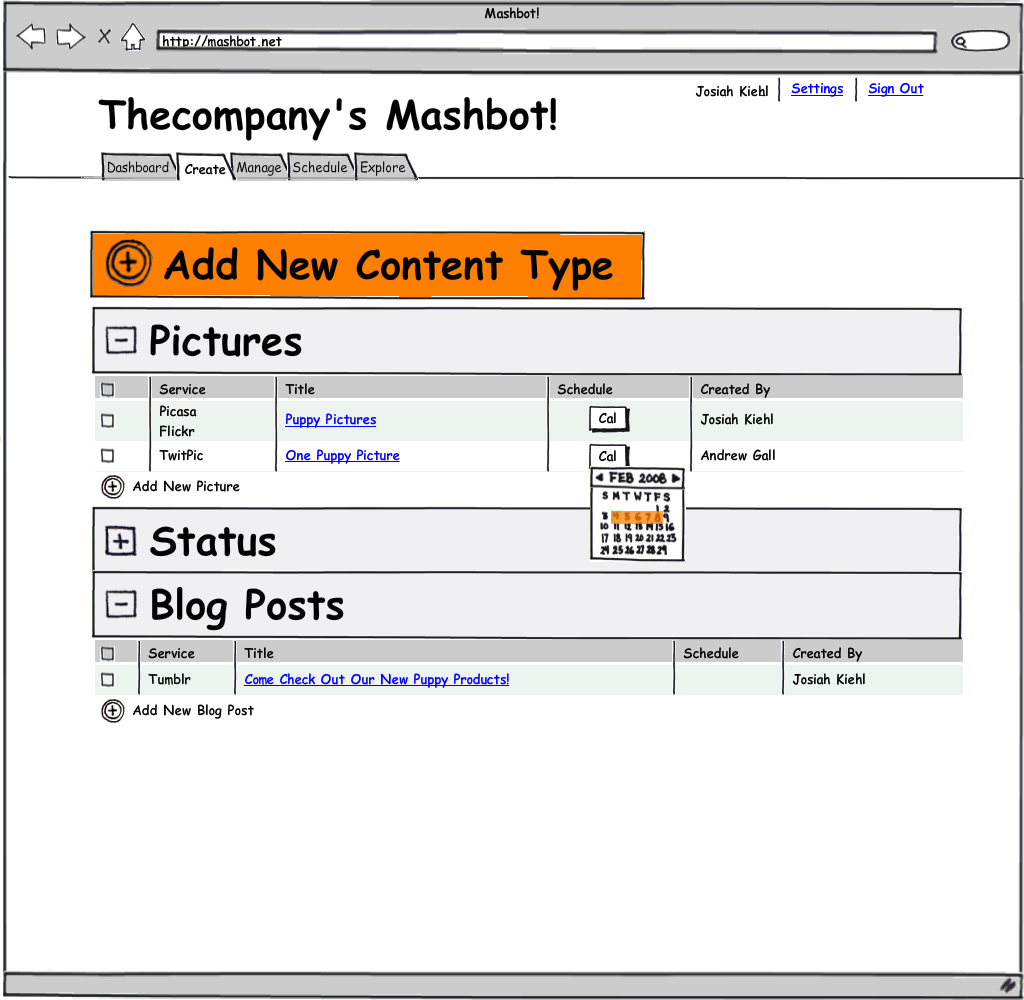
\includegraphics[width=\textwidth]{../mockups/create.png}
Given pojo is logged in \\
When I go to the create campaign page \\
And I fill in ``Amazing Campaign'' for ``Title'' \\
And I fill in ``01/15/2100'' for ``Start date'' \\
And I fill in ``02/14/2100'' for ``End date''   \\
And I press ``Create!'' \\
Then I should see ``Amazing Campaign'' \\
And I should see ``01/15/2100'' \\
And I should see ``02/14/2100'' \\

Scenario: Creating a campaign \\
Given pojo is logged in \\
When I go to the create campaign page \\
And I fill in ``Unfail Campaign'' for ``Title'' \\
And I press ``Create!'' \\
Then I should see ``Unfail Campaign'' \\

Scenario: Validate sane start and end dates: start should be before end. \\
Given pojo is logged in \\
When I go to the create campaign page \\
And I fill in ``Fail Campaign'' for ``Title'' \\
And I fill in ``01/15/2100'' for ``Start date'' \\
And I fill in ``01/14/2100'' for ``End date'' \\
And I press ``Create!'' \\
Then I should see ``Hold up! You can't end something before you start it!'' \\

Scenario: Make sure you can't have an end date without a start date. \\
Given pojo is logged in \\
When I go to the create campaign page \\
And I fill in ``Fail Campaign'' for ``Title'' \\
And I fill in ``01/14/2100'' for ``End date'' \\
And I press ``Create!'' \\
Then I should see ``Whoa buddy! You're going to need a start date if you intend to have an end date'' \\
\end{hangparas}

\subsubsection{Feature: Schedule Campaign}

\begin{hangparas}{0.25in}{1}
Feature: Schedule Campaign \\
In order to schedule campaigns \\
As a user \\
I want to schedule and manage the start and end time of campaigns. \\

Scenario: Unscheduled Campaign List \\
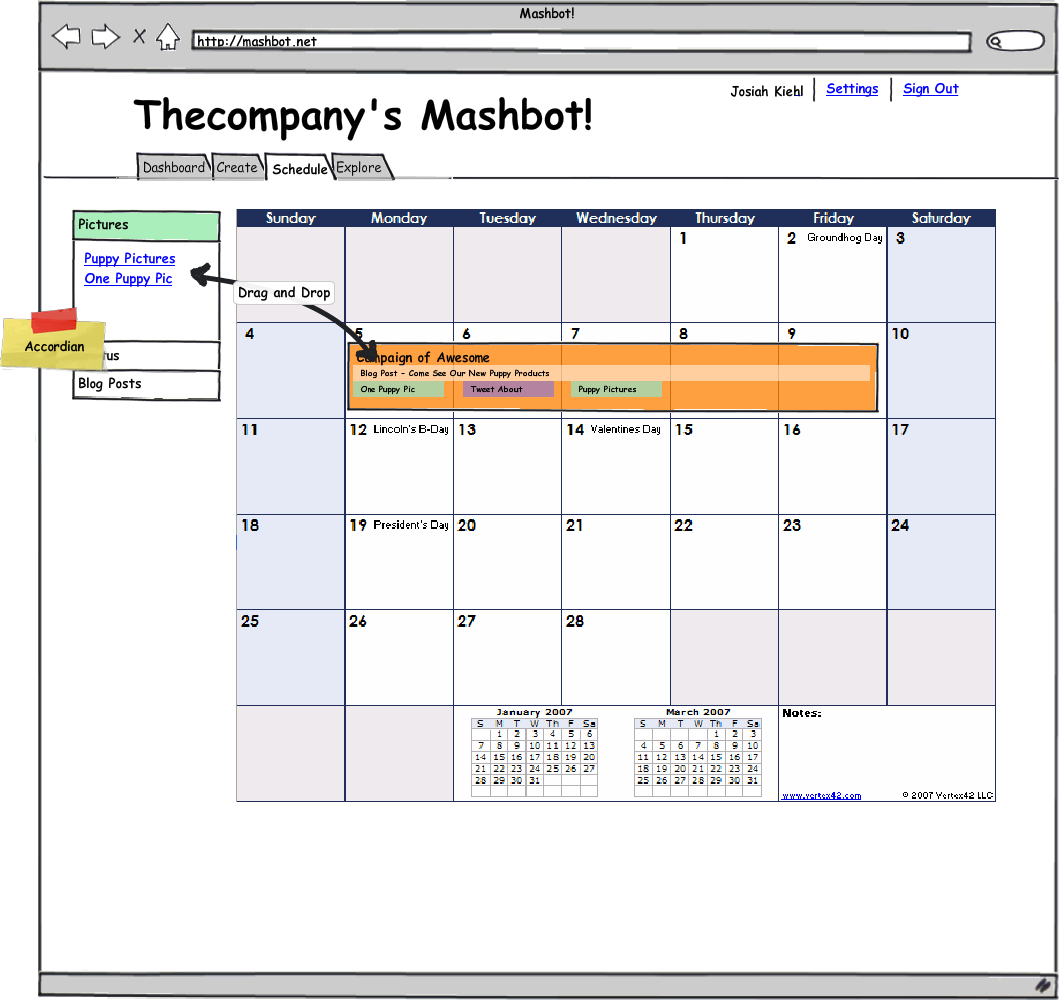
\includegraphics[width=\textwidth]{../mockups/schedule.png}
  Given pojo is logged in \\
  And I have campaigns titled Twitterblast, Social Network Blitz \\
  When I go to the schedule page \\
  Then I should see ``Twitterblast'' \\
  And I should see ``Social Network Blitz'' \\
  
Scenario: Create a new blog post \\
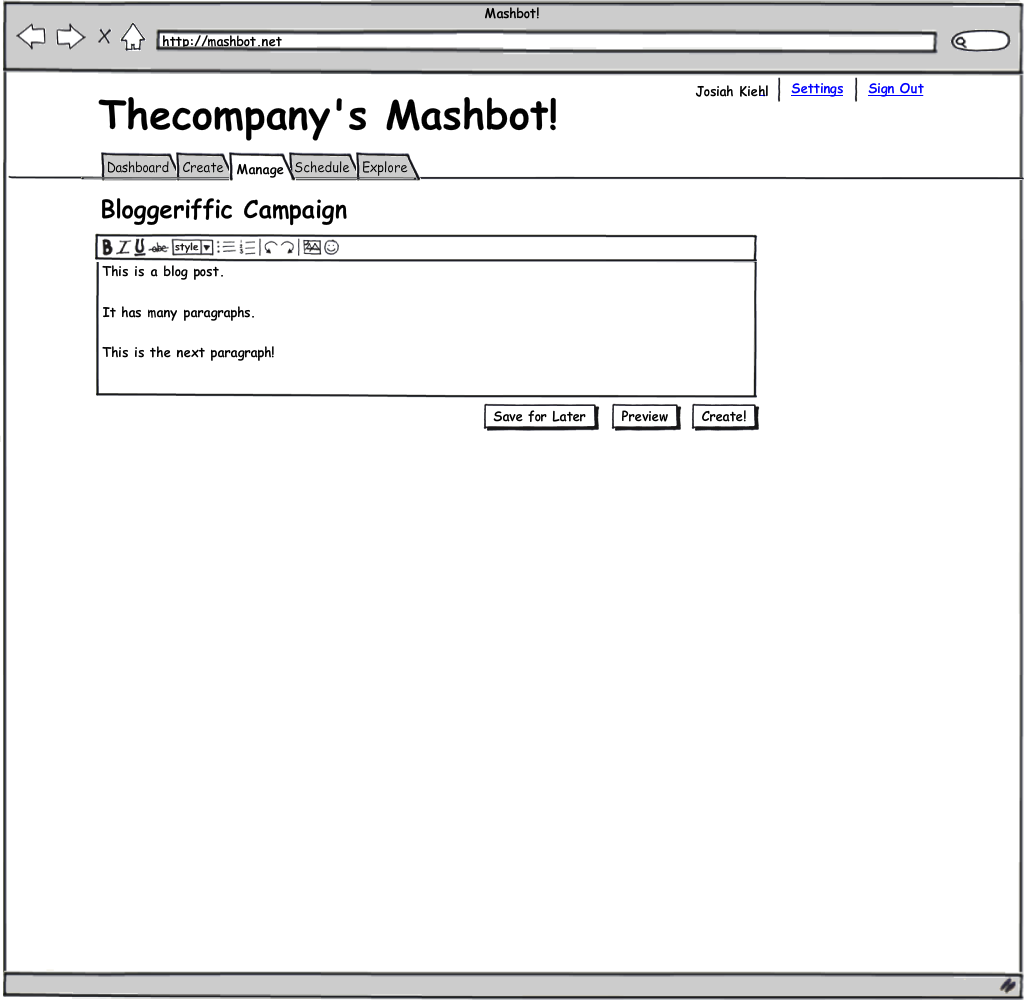
\includegraphics[width=\textwidth]{../mockups/manage-create-blog-post.png}
  Given jsmith is logged in \\
  When I go to the create text post page \\
  And I fill in ``My new blog!'' for ``Title''
  And I fill in ``I'm so awesome.. listen to me!'' for ``Body'' 
  And I press ``Create!'' 
  Then I should see ``My new blog!'' 
  
Scenario: Create a new photo post \\
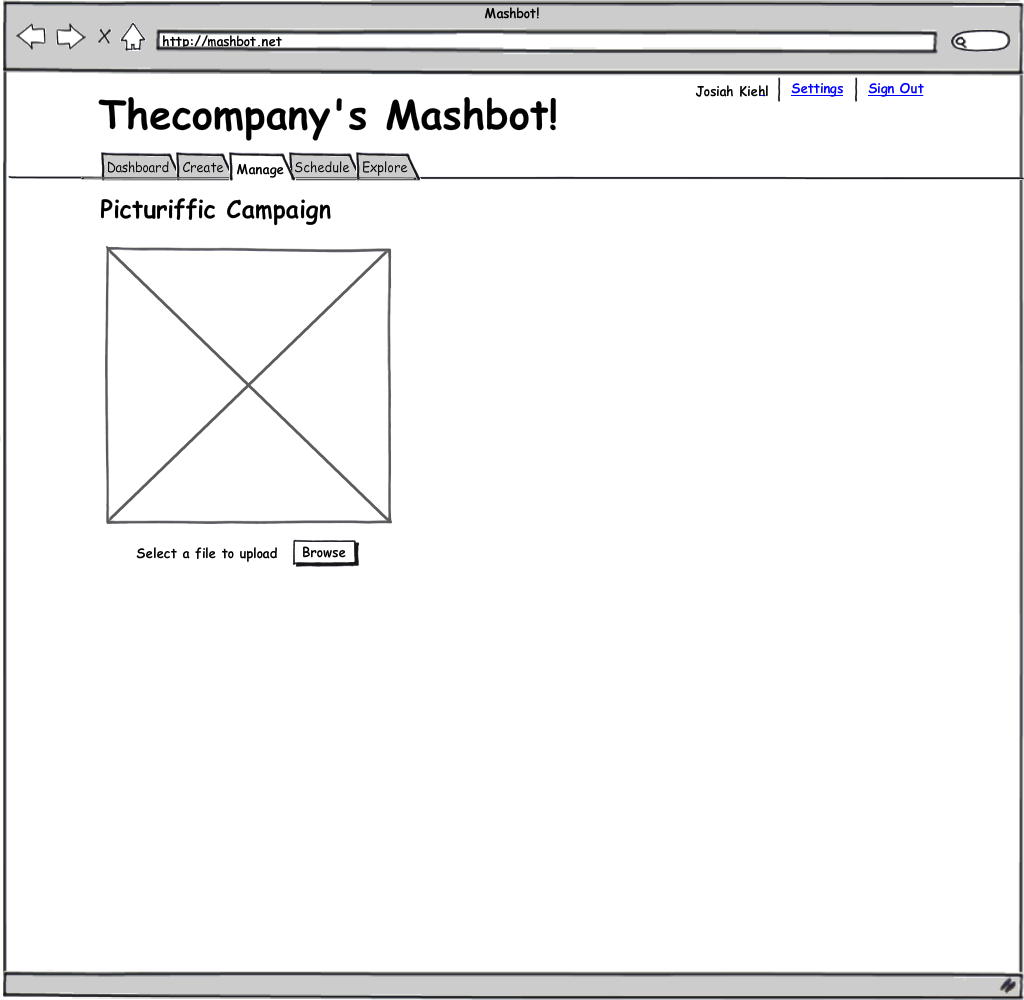
\includegraphics[width=\textwidth]{../mockups/manage-create-image.png}
  Given jsmith is logged in \\
  When I go to the create photo post page \\
  And I fill in ``ACME in London'' \\
  And I upload an image file in ``Photo'' \\
  And I fill in ``travel, london'' for ``Tags'' \\
  And I press ``Create!'' \\
  Then I should see ``XYZ Corp in London'' \\
  
  Scenario: Create a new video post \\
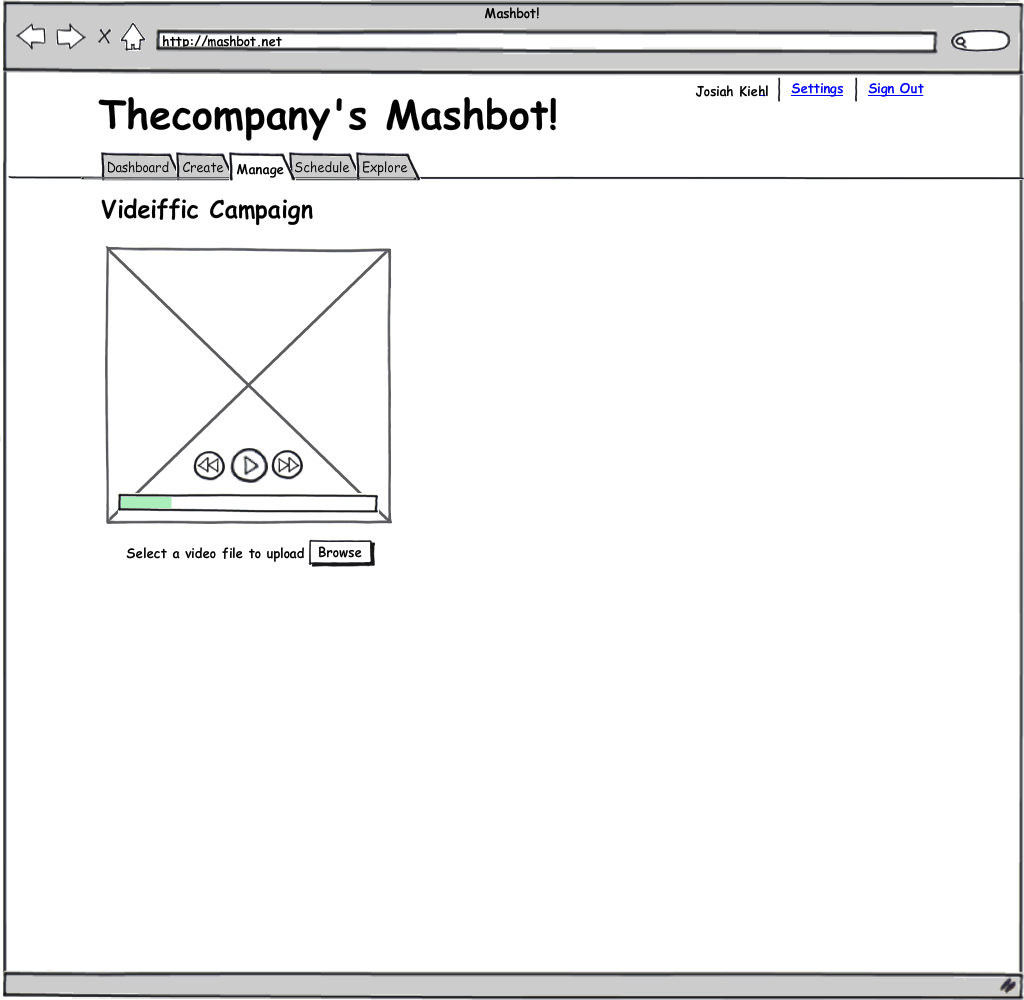
\includegraphics[width=\textwidth]{../mockups/manage-create-video.png}
    Given jsmith is logged in \\
    When I go to the create video post page \\
    And I fill in ``ACME's new Widget'' \\
    And I upload a video file in ``Video'' \\
    And I press ``Create!'' \\
    Then I should see ``ACME's new Widget'' \\
  
  Scenario: Create a new status post \\
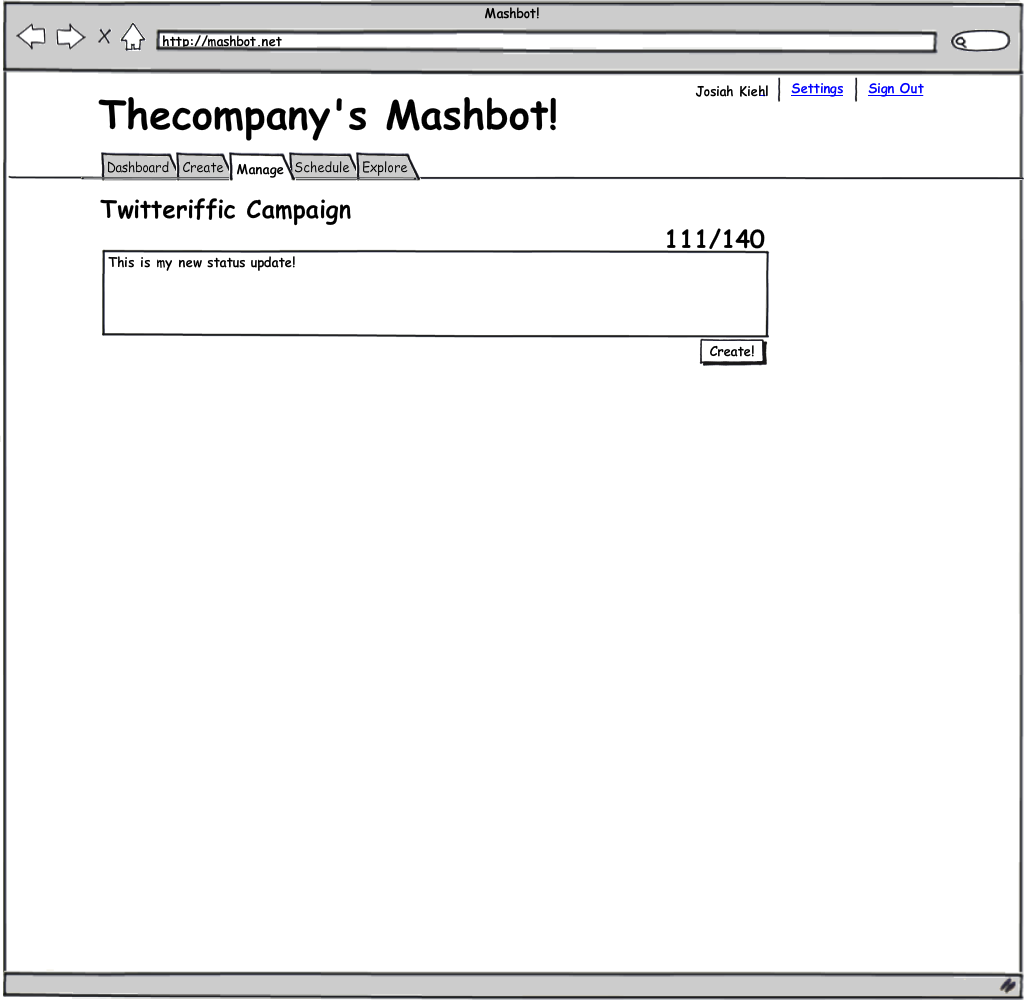
\includegraphics[width=\textwidth]{../mockups/manage-create-status-update.png}
    Given jsmith is logged in \\
    When I go to the create status post page \\
    And I fill in ``Visiting a new client in Beijing.'' \\
    And I upload a video file in ``Status'' \\
    And I press ``Create!'' \\
    Then I should see ``Visiting a new client in Beijing.'' \\

  Scenario: Schedule a blog post \\
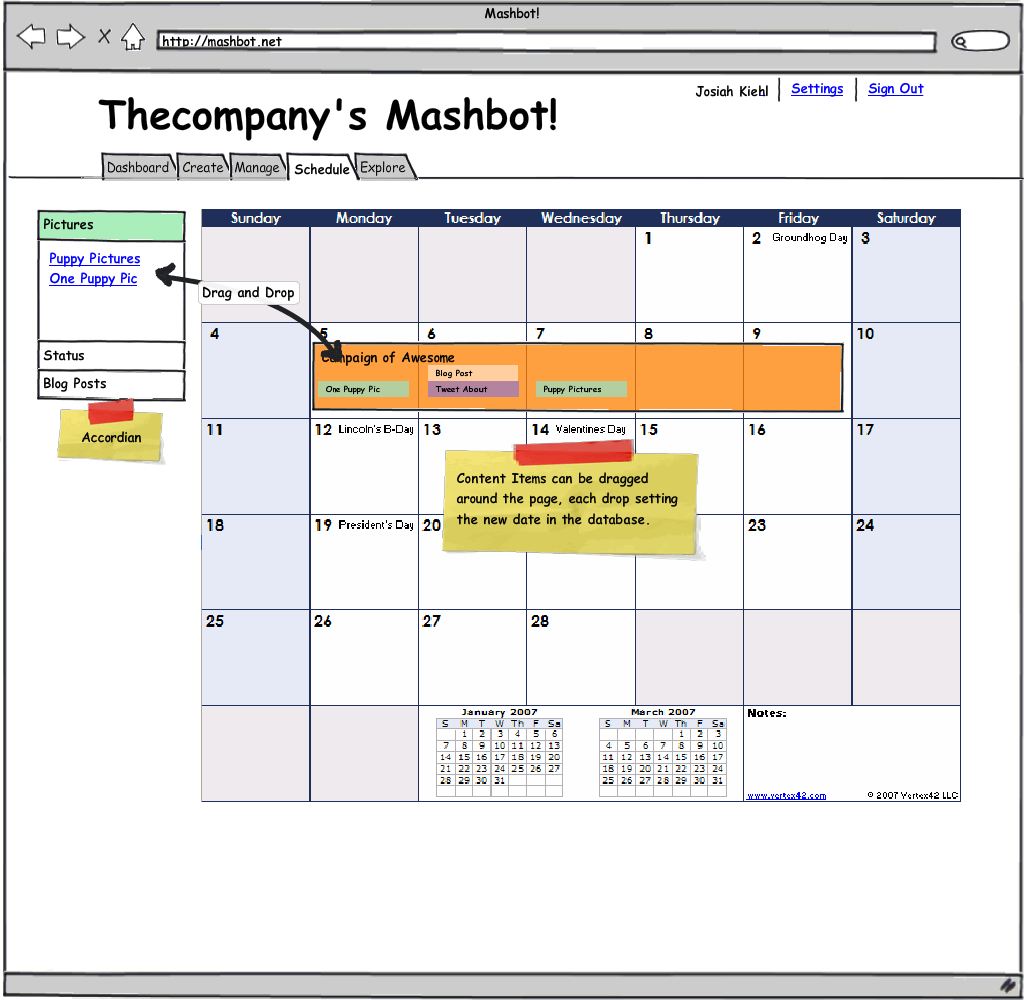
\includegraphics[width=\textwidth]{../mockups/schedule-content.png}
    Given jsmith is logged in \\
    And there is a blog post with the title ``My new blog!'' \\
    When I go to the schedule page \\
    And I click ``Schedule'' \\
    And I fill in ``02/20/10'' for ``Date''
    And I fill in ``01:23'' for ``Time''
    And I press ``Schedule!'' 
    Then the blog post with the title ``My new blog!'' is saved with a ``Publish Time'' of ``1266628980'' 
\end{hangparas}

\end{document}
